\chapter{Sum-product networks}\label{chp:spn}

In this chapter we provide some background concepts needed for defining a sum-product network. Once
this is covered, we formally define an SPN, list some interesting properties on their structure,
and describe how to perform exact inference (i.e.\ extract the probability of evidence of some
valuation) and how to find an approximation of the maximum a posteriori probability.

We leave all proofs in~\autoref{app:proofs}.

\section{Background}

The objective of probabilistic modelling is to compactly represent a probability distribution, be
able to find a good approximation to the real function and be able to efficiently compute both
the marginals and modes. Probabilistic graphical models (PGMs) attempt to solve this through the
use of graphs, representing distributions as a normalized product of factors (\cite{pearl-1988}).
\begin{equation*}
  P(X=x)=\frac{1}{Z}\prod_k \phi_k(x_{\{k\}})
\end{equation*}

Where $x\in\mathcal{X}$ is a $d$-dimensional vector valuation of RVs $\mathbf{X}$ on sample space
$\mathcal{X}$, and factor (also called a potential) $\phi_k$ is a function mapping instantiations
of $X$ to a non-negative number. $Z$ is the partition function $Z=\sum_{x\in\mathcal{X}} \prod_k
\phi_k(x_{\{k\}})$ that sums out all variables and normalizes the term above it to the $[0,1]$
range.

A downside of this representation is that inference is exponential on the worst case, which makes
learning also exponential, as it uses inference as a subroutine. To get around this problem,
Darwiche proposed in~\cite{diff-approach-darwiche} the notion of \textit{network polynomial}.

A network polynomial is a function over the probabilities of each instantiation. Let $\Phi(x)$ be a
probability distribution. The network polynomial of $\Phi(x)$ is the function
$f=\sum_{x\in\mathcal{X}}\Phi(x)\Pi(x)$, where $\Pi(x)$ is the product of the IVs of each variable
on instantiation $x$, where each indicator variable $[Y=y]$ has a value of zero if $Y\neq y$ in $x$
and a value of one otherwise (i.e.\ if $Y=y$ in $x$ or $Y\not\in x$).

As an example, take the bayesian network $\mathcal{N}=A\to B$ with binary variables. Let
$\lambda_a$, $\lambda_{\ov{a}}$, $\lambda_b$ and $\lambda_{\ov{b}}$ be the indicator variables for
when $A=1$, $A=0$, $B=1$ and $B=0$ respectively. The network polynomial of $\mathcal{N}$ is the
expression
\begin{equation*}
  f_{\mathcal{N}}=P(a)P(b|a)\lambda_a\lambda_b+P(a)P(\ov{b}|a)\lambda_a\lambda_{\ov{b}}+
  P(\ov{a})P(b|\ov{a})\lambda_a\lambda_{\ov{b}}+P(\ov{a})P(\ov{b}|\ov{a})\lambda_{\ov{a}}
  \lambda_{\ov{b}}.
\end{equation*}

The main advantage of this representation is to avoid recomputing terms. For instance, take an
instantiation of $x=\{A=0\}$. Then, the network polynomial will be as follows.
\begin{align*}
  f_{\mathcal{N}}(x)&=P(a)P(b|a)\cdot 0\cdot 1+P(a)P(\ov{b}|a)\cdot 0\cdot
  1+P(\ov{a})P(b|\ov{a})\cdot 1\cdot 1+P(\ov{a})P(\ov{b}|\ov{a})\cdot 1\cdot 1=\\
  &=P(\ov{a})P(b|\ov{a})+P(\ov{a})P(\ov{b}|\ov{a})
\end{align*}

Which means we can avoid computing values from the two first terms. We can also compute the network
polynomial of some unnormalized probability distribution as long as we divide by the partition
function, defined as the network polynomial with all indicators set to one. Although the network
polynomial has exponential size in terms of variables, computing the probability of evidence is
linear in its size. By representing the network polynomial as an arithmetic circuit of sums and
products, one can prove that the cost of inference is indeed polynomial.

\section{Definitions and properties}

Sum-product networks borrow many concepts from network polynomials and arithmetic circuits. There
are many definitions of SPNs and in this thesis we present two. The first definition is given by
the seminal article~\cite{poon-domingos}, and can be seen as a more low-level approach to defining
the network\@. The second, based on~\cite{gens-domingos}, is a stronger definition, but one which
we will use more throughout this thesis, as it lends itself better to continous data.

Let $\mathbf{X}=\{X_1,X_2,\ldots,X_n\}$ be the set of all variables. We shall call this set the
root scope. Let $G$ be a graph $G$. The sets of vertices and edges of $G$ will be denoted by $V(G)$
and $E(G)$. We will call $\Ch(n)$ and $\Pa(n)$ the sets of children and parents of node $n\in
V(G)$.

\begin{figure}[h]
  \centering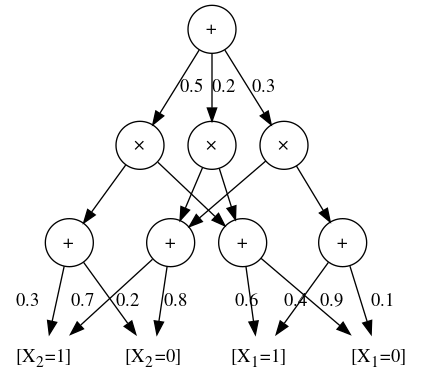
\includegraphics[scale=0.6]{graphs/sample_spn.png}
  \caption{An example of an SPN.\label{fig:sample_spn}}
\end{figure}

\begin{definition}[Sum-product network;~\cite{poon-domingos}]
  A sum-product network (SPN) over variables $X_1,X_2,\ldots,X_n$ is a DAG whose leaves are
  indicator variables $[X_1=x_1^1],[X_2=x_2^1],\ldots,[X_n=x_n^1],\ldots,[X_1=x_1^d],[X_2=x_2^d],
  \ldots,[X_n=x_n^d]$. Its internal nodes are weighted sums or products. Each edge coming out from
  a sum node $n$ to another node $j$ has a non-negative weight associated with it. We denote such
  weight by $w_{n,j}$. The value of a sum node $n$ is $v_n=\sum_{j\in\Ch(n)}w_{n,j}v_j$, where
  $v_j$ is the value of node $j$. The value of a product node $n$ is $v_n=\prod_{j\in\Ch(n)}v_j$.
  The value of a leaf node is the value of the indicator variable. The value of the SPN is the
  value of its root node.
\end{definition}

Throughout this thesis, we denote by $S(X=x)$ the value of an SPN $S$ given evidence $x$. A sub-SPN
$S_n$ of $S$ is the subgraph of $S$ rooted at $n$. A node in an SPN is itself an SPN\@. When all
indicator variables are set to one, the value of $S$ is denoted by $S(\ast)$. The scope of an SPN
$S$, denoted by $\Sc(S)$, is the union set of all scopes of its children. A leaf's scope is the
scope of its IV\@.

\begin{definition}[Validity]
  An SPN is valid iff, for all evidence $E=e$, $S(E=e)=\Phi_S(E=e)$, where $\Phi_S$ is an
  unnormalized probability distribution.
\end{definition}

\begin{definition}[Completeness]
  An SPN is complete iff all children of the same sum node have the same scope.
\end{definition}

\begin{definition}[Consistency]
  An SPN is consistent iff no variable appears with a value $v$ in one child of a product node and
  valued $u$, with $u\neq v$, in another.
\end{definition}

Validity in an SPN means that the network correctly and efficiently computes the probability of
evidence of the distribution it represents. In this document we only work with valid SPNs, as we
wish to always compute exact inference. However, non-valid SPNs are an interesting field of
research for approximate inference in SPNs.

A sufficient condition for validity is completeness and consistency. Yet whilst this condition is
sufficient, it is not necessary, as the converse (i.e.\ an incomplete and inconsistent valid SPN)
can hold.

\begin{theorem}[\cite{poon-domingos}]
  An SPN is valid if it is complete and consistent.
\end{theorem}

When an SPN $S$ is valid, then $S(\ast)$ is the partition function, and we can extract the
probability of evidence from an SPN by computing $P(X=x)=S(x)/S(\ast)$. If for every sum node all
of their weights are non-negative and sum to one, then the partition function is $S(\ast)=1$, and
the SPN is the distribution itself.

\begin{corollary}[Validity recursion;~\cite{poon-domingos}]
  If an SPN $S$ is valid, then all sub-SPN of $S$ is valid.
\end{corollary}

\begin{definition}[Decomposability]
  An SPN is decomposable iff no variable appears in more than one child of a product node.
\end{definition}

In other words, an SPN is decomposable if and only if, for every product node, every child node has
disjoint scopes with relation to all their other siblings. It is easy to see that decomposability
implies in consistency, as there can be no inconsistency between product children since scopes are
disjoint. Therefore, a complete and decomposable SPN is valid. Indeed it is much easier to produce
decomposable SPNs then only consistent ones, and although this condition may seem too strong and
restrictive,~\cite{theoretical-spn} showed that a consistent SPN is representable by a polynomially
larger decomposable SPN\@.

So far, SPNs are restricted to the discrete domain, as we rely on IVs to define possible valuations
to variables. We can generalize SPNs to the continuous by assuming an infinite number of IVs and
thus replacing sum nodes whose children are IVs with integral nodes. A leaf node then becomes an
integral node with infinite IVs as children. Particularly, it represents an unnormalized
univariate probability distribution, such as a Gaussian. The value of this integral node $n$
becomes the pdf $p_n(x)$. This extension brings us to a second definition of SPNs.

\begin{definition}[Sum-product networks;~\cite{gens-domingos}]
  A sum-product network is defined recursively as follows.
  \begin{enumerate}[noitemsep]
    \item A tractable univariate probability distribution is an SPN\@.
    \item A product of SPNs with disjoint scopes is an SPN\@.
    \item A weighted sum of SPNs with the same scope is an SPN, provided all weights are positive.
    \item Nothing else is an SPN\@.
  \end{enumerate}
\end{definition}

This second definition limits our scope to only complete and decomposable SPNs. Note that an IV is
also an SPN, as we can assume that an indicator variable is a degenerate tractable univariate
distribution, taking a value of one if it agrees with the given evidence and zero otherwise.

\section{Inference}

Throughout this thesis we assume that all sum nodes are normalized and sum to one, meaning the
partition function is $S(\ast)=1$ and the SPN's value is the probability itself.

Let $X=\{X_1=x_1,X_2=x_2,\ldots,X_k=x_k\}$ be a valuation and $S$ be an SPN\@. We say that $X$ is a
complete valuation if $\Sc(X)=\Sc(S)$. That is, $X$ contains a valuation for all variables in $S$.
An incomplete valuation has some variable assignment missing.

Computing the probability of evidence is done through a bottom-up backwards pass through the SPN\@.
To find the value of an SPN, we must know the value of the root node, which depends on all nodes
below it. This is done through a topological traversal of the graph.

Finding the value of a leaf node depends on the valuation given. Let $n$ be a leaf node, and
$\Sc(n)=\{X_j\}$. Let $X$ be some valuation. Assuming the univariate probability distribution of
$n$ has fpd $p_n(x)$, then if $X$ has a valution $X_j=x_j$, the value of node $n$ will be
$S_n(X)=p_n(x_j)$. If $X$ has no valuation for variable $X_j$, then $S_n(X)$ is the
distribution's mode. Note that this holds for indicator variables, as if $X$ has a valuation for
$X_j=x_j$ and the IV matches with $x_j$, then $p_n(x_j)=1$. In case it does not, $p_n(x_j)=0$. For
the incomplete case, the mode of an indicator variable is one, which holds the equivalence.

Once we compute leaf nodes, we can compute each internal node's values by following the topological
order until we reach the root. For sum nodes, we compute the weighted sum
$S_n(X)=\sum_{j\in\Ch(n)}w_{n,j}S_j(X)$, and for products $S_n(X)=\prod_{j\in\Ch(n)}S_j(X)$.

\begin{figure}[h]
  \centering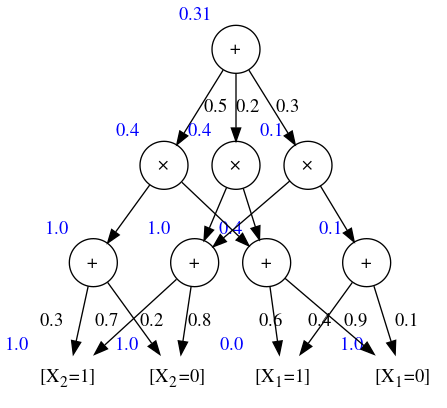
\includegraphics[scale=0.6]{graphs/sample_spn_prob.png}
  \caption{Computing the probability of evidence on a sample SPN.\label{fig:sample_spn_prob}}
\end{figure}

\autoref{fig:sample_spn_prob} shows the value of the SPN in \autoref{fig:sample_spn} given a
valuation $X=\{X_1=0\}$. Values in blue are the values of each sub-SPN\@. Finding the probability
of evidence $P(X=x)$ is fast, as computing the value of an SPN is linear to the number of edges of
the graph.

Additionally, we might want to find the probability that maximizes a certain valuation, i.e.\ the
maximum a posteriori probability (MAP). To compute the approximate value of the MAP of some
valuation $X$, we first transform the SPN into a max-product network (MPN) by replacing all sums
with max nodes. The value of a max node is the maximum value of its weighted children. More
formally, the value of an MPN's max node $n$ is given by $M_n(X)=\max_{j\in\Ch(n)} w_{n,j}M_j(X)$.
Other nodes behave identically to an SPN\@. The computed value of an MPN is an approximation of
$\max_y P(X=x, Y=y)$, where $X$ is incomplete and $Y$ is the set of variables that are missing.
This is called the max-product algorithm.

In SPNs, computing the exact MAP was shown to be NP-hard (\cite{theoretical-spn,cmc2017,mei2018}),
and better approximation algorithms were proposed as an alternative to the max-product algorithm
described here. However, in this thesis, when we talk about computing the (approximate) MAP, we are
referring to the usual max-product algorithm.

\begin{figure}[h]
  \centering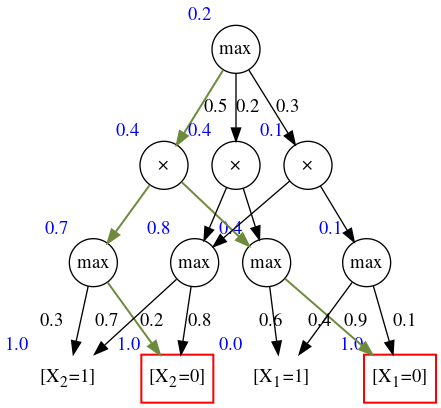
\includegraphics[scale=0.6]{graphs/sample_mpn_prob.png}
  \caption{Computing the approximate MAP of an SPN through its MPN.\label{fig:sample_mpn_prob}}
\end{figure}

Once the MPN values are computed, we can find the most probable explanation (MPE) of the
distribution given an evidence. This is done through a top-down forward pass, where we take a
maximum sub-circuit path of the MPN by always taking the max path at a max node and taking all
paths on a product node. The MPE are the maximum sub-circuit leaves' instantiations.

\autoref{fig:sample_mpn_prob} shows the MPN of the SPN shown in \autoref{fig:sample_spn} given
$X=\{X_1=0\}$, where the numbers in blue represent the MPN values at each node, green arrows
indicate the sub-circuit of maximum value and red boxes indicate the most probable valuations given
evidence. The resulting MPE $\argmax_{y\in\mathcal{Y}} P(X=\{X_1=0\},Y=y)$ is the valuation
$\{X_1=0, X_2=0\}$.

Therefore, computing the probability of evidence, which is also called \textit{soft} inference, of
an SPN is done through a single bottom-up pass. Similarly, computing the MAP probability, refered
to as \textit{hard} inference, is done through a bottom-up pass on the SPN's MPN\@.  On the other
hand, finding the MPE valuations requires a bottom-up pass to first compute the MAP, and then a
top-down search to find the most probable instantiations.

We provide next pseudocode for computing both soft and hard inference. We assume as input only
valid, (weight) normalized SPNs. However, one could easily extend the included algorithms for
unnormalized networks.

\begin{algorithm}[H]
  \caption{\code{SoftInference}: Computes the probability of evidence in SPNs}
  \begin{algorithmic}[1]
    \Require\, A valid SPN $S$ with normalized weights and a valuation $X$
    \Ensure\, The soft inference values at each node $S_n$
    \State\, Initialize $S_n=0$
    \State\, Find topological order $T$ of $S$
    \For{each node $n\in S$ from $T$}
      \If{$n$ is a leaf node}
        \State\, Let $\Sc(n)=\{X_k\}$, $p_n(x)$ be $n$'s pdf and $\hat{p}_n$ be $p_n$'s mode
        \If{$X_k\in X$}
          \State\, Let $x_k$ be $X_k$'s value in $X$
          \State\, $S_n\gets p_n(x_k)$
        \Else%
          \State\, $S_n\gets\hat{p}_n$
        \EndIf%
      \ElsIf{$n$ is sum node}
        \For{all $j\in\Ch(n)$}
          \State\, $S_n\gets S_n + w_{n,j}S_j$
        \EndFor%
      \Else%
        \For{all $j\in\Ch(n)$}
          \State\, $S_n\gets S_n\cdot S_j$
        \EndFor%
      \EndIf
    \EndFor%
    \State\,\textbf{return} each $S_n$ node value
  \end{algorithmic}
\end{algorithm}

\begin{algorithm}[H]
  \caption{\code{HardInference}: Computes an approximation of the MAP in SPNs}
  \begin{algorithmic}[1]
    \Require\, A valid SPN $S$ with normalized weights and a valuation $X$
    \Ensure\, The hard inference values at each node $M_n$
    \State\, Let $M$ be $S$'s MPN
    \State\, Initialize $M_n=0$
    \State\, Find topological order $T$ of $M$
    \For{each node $n\in M$ from $T$}
      \If{$n$ is a leaf node}
        \State\, Let $\Sc(n)=\{X_k\}$, $p_n(x)$ be $n$'s pdf and $\hat{p}_n$ be $p_n$'s mode
        \If{$X_k\in X$}
          \State\, Let $x_k$ be $X_k$'s value in $X$
          \State\, $M_n\gets p_n(x_k)$
        \Else%
          \State\, $M_n\gets\hat{p}_n$
        \EndIf%
      \ElsIf{$n$ is sum node}
        \For{all $j\in\Ch(n)$}
          \State\, $M_n\gets\max(M_n, w_{n,j}M_j)$
        \EndFor%
      \Else%
        \For{all $j\in\Ch(n)$}
          \State\, $M_n\gets M_n\cdot M_j$
        \EndFor%
      \EndIf
    \EndFor%
    \State\,\textbf{return} each $M_n$ node value
  \end{algorithmic}
\end{algorithm}

Finally, we show how to algorithmically compute the MPE given some evidence.

\begin{algorithm}[H]
  \caption{\code{ArgMaxSPN}: Finds the MPE of a valuation on an SPN}
  \begin{algorithmic}[1]
    \Require\, A valid SPN $S$ with normalized weights and a valuation $X$
    \Ensure\, The $\argmax$ values of each variable according to $X$
    \State\, $M\gets$\code{HardInference}$(S, X)$
    \State\, Let $Y$ be a copy of $X$
    \State\, Let $Q$ be a queue
    \State\, Push $S$ into $Q$
    \For{each node $n\in M$ in $Q$}
      \If{$n$ is a leaf node}
        \State\, Let $\Sc(n)=\{X_k\}$ and $p_n(x)$ be $n$'s pdf
        \State\, Let $\hat{x}=\argmax_{x_k} p_n(x_k)$ be $p_n$'s maximum valuation
        \If{$X_k\not\in X$}
          \State\, $Y\gets Y\cup\{X_k=\hat{x}\}$
        \EndIf%
      \ElsIf{$n$ is sum node}
        \State\, Push maximum child $M_j$, $j\in\Ch(n)$ into $Q$
      \Else%
        \State\, Push all children $j\in\Ch(n)$ into $Q$
      \EndIf
    \EndFor%
    \State\,\textbf{return} Y
  \end{algorithmic}
\end{algorithm}
